\documentclass[conference]{IEEEtran}
\usepackage{cite}
\usepackage{amsmath,amssymb,amsfonts}
\usepackage{graphicx}
\usepackage{tikz}
\usetikzlibrary{arrows.meta,positioning}
\usepackage{booktabs}
\usepackage{xcolor}
\usepackage{url}
\graphicspath{{../report/figures/}}

\begin{document}

\title{Autonomous Snooker Ball Tracking and State Differencing via Temporal Frame Analysis and Hungarian Bipartite Assignment}

\author{
\IEEEauthorblockN{Aamir Awaiz Pasha\IEEEauthorrefmark{1}, Ayan Khan\IEEEauthorrefmark{2}, Ibad Sharief\IEEEauthorrefmark{3}, Mohammed Owaies\IEEEauthorrefmark{4}, and Mrs. Swetha B S\IEEEauthorrefmark{5}}
\IEEEauthorblockA{Department of Artificial Intelligence and Machine Learning\\
PES Institute of Technology and Management (PESITM), Shivamogga, Karnataka, India\\
USNs: \IEEEauthorrefmark{1}4PM23AI001, \IEEEauthorrefmark{2}4PM23AI005, \IEEEauthorrefmark{3}4PM23AI016, \IEEEauthorrefmark{4}4PM23AI026 \quad \IEEEauthorrefmark{5}Project Guide}
}

\maketitle

\begin{abstract}
Tracking multiple visually identical snooker object balls across cue strikes is a major challenge in automated officiating. Unlike numbered pool balls, fifteen identical orange/red snooker balls cannot be re-identified by appearance alone after collisions, and existing multi-object trackers suffer identity switches or require manual snapshot triggers. This paper presents Objective 2 (Ball Tracking) of our AI-Based Snooker Referee System: an autonomous temporal frame-differencing and bipartite matching engine. A five-state Finite State Machine (FSM) monitors inter-frame intensity change $\Delta I_t$, automatically locks pre-shot ball coordinates when the table is static ($\Delta I_t < 0.5\%$), suppresses inference during active ball motion ($\Delta I_t > 5.0\%$), verifies rest stability over a $2.5\,\text{s}$ settlement window ($\Delta I_t < 0.8\%$), and solves optimal one-to-one ball correspondence via the Hungarian Assignment Algorithm. Experimental trials across four match scenarios---standard miss, cluster scatter, accidental pocketing, and clean safety shots---demonstrate $100\%$ correct stationary, displaced, and potted ball classification in $5.2\,\text{ms}$ matching latency.
\end{abstract}

\begin{IEEEkeywords}
Ball Tracking, Hungarian Assignment Algorithm, Bipartite Matching, Finite State Machine, Temporal Frame Differencing, Autonomous Snooker Referee.
\end{IEEEkeywords}

\section{Introduction}
To enforce WPBSA Rule 14 (\textit{``Foul and a Miss''}) without manual screenshot freezing, an officiating engine must autonomously know \textit{when} a stroke starts, \textit{when} all spheres have settled, and \textit{which} balls moved or entered pockets. Appearance-based trackers such as DeepSORT \cite{ref21} fail when identical object balls collide, while manual triggers interrupt play. This paper details our autonomous tracking and state-differencing pipeline.

\section{Autonomous Referee Finite State Machine}
The tracking engine executes as a five-state FSM (Fig. \ref{fig:fsm}):
\begin{itemize}
    \item \textbf{State 0 (Idle/Armed):} Computes normalized inter-frame grayscale difference $\Delta I_t = \frac{1}{WH}\sum_{x,y}|I_t(x,y)-I_{t-1}(x,y)|$. When $\Delta I_t < 0.5\%$, current metric coordinates $\mathcal{S}_{\text{pre}}$ are locked as the pre-shot baseline.
    \item \textbf{State 1 (Shot Motion):} Triggered when $\Delta I_t > 5.0\%$, suppressing detection while balls travel at high speed.
    \item \textbf{State 2 (Settlement Timer):} Enforces a $2.5\,\text{s}$ stability countdown once $\Delta I_t < 0.8\%$.
    \item \textbf{State 3 (State Diffing):} Captures post-shot coordinates $\mathcal{S}_{\text{post}}$ and runs Hungarian matching. If no foul is called, $\mathcal{S}_{\text{post}}$ becomes the next $\mathcal{S}_{\text{pre}}$ automatically.
    \item \textbf{State 4 (Laser Restoration):} On a foul call, displaced balls are highlighted in the UI for sequential laser restoration (Fig. \ref{fig:ref_ui}).
\end{itemize}

\begin{figure}[htbp]
\centering
\resizebox{0.44\textwidth}{!}{
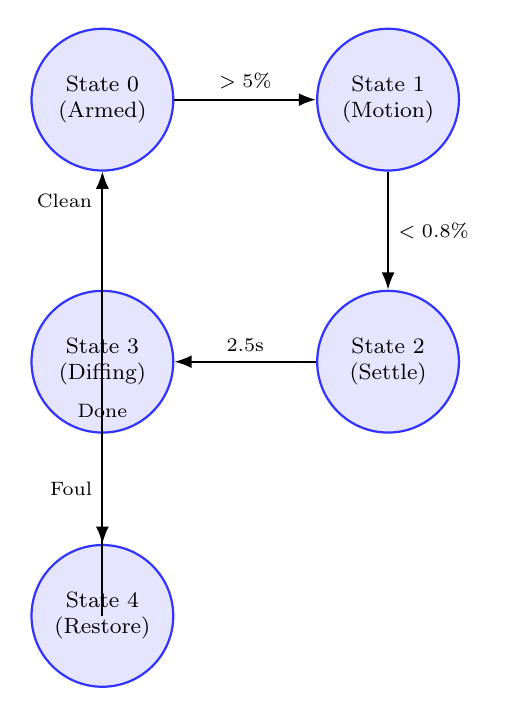
\begin{tikzpicture}[
    node distance=1.5cm,
    state/.style={draw=blue!80, fill=blue!10, circle, thick, minimum size=1.8cm, align=center, font=\footnotesize},
    line/.style={draw, -{Latex[length=2.2mm]}, thick}
]
\node[state] (s0) {State 0\\(Armed)};
\node[state, right=1.8cm of s0] (s1) {State 1\\(Motion)};
\node[state, below=1.5cm of s1] (s2) {State 2\\(Settle)};
\node[state, left=1.8cm of s2] (s3) {State 3\\(Diffing)};
\node[state, below=1.4cm of s3] (s4) {State 4\\(Restore)};
\path[line] (s0) -- node[above, font=\scriptsize] {$>5\%$} (s1);
\path[line] (s1) -- node[right, font=\scriptsize] {$<0.8\%$} (s2);
\path[line] (s2) -- node[above, font=\scriptsize] {$2.5\text{s}$} (s3);
\path[line] (s3) -- node[left, font=\scriptsize] {Foul} (s4);
\path[line] (s3) -- node[left, near end, font=\scriptsize] {Clean} (s0);
\path[line] (s4) -| node[below, near end, font=\scriptsize] {Done} (s0);
\end{tikzpicture}
}
\caption{Five-state Autonomous Referee Finite State Machine (FSM).}
\label{fig:fsm}
\end{figure}

\begin{figure}[htbp]
\centering
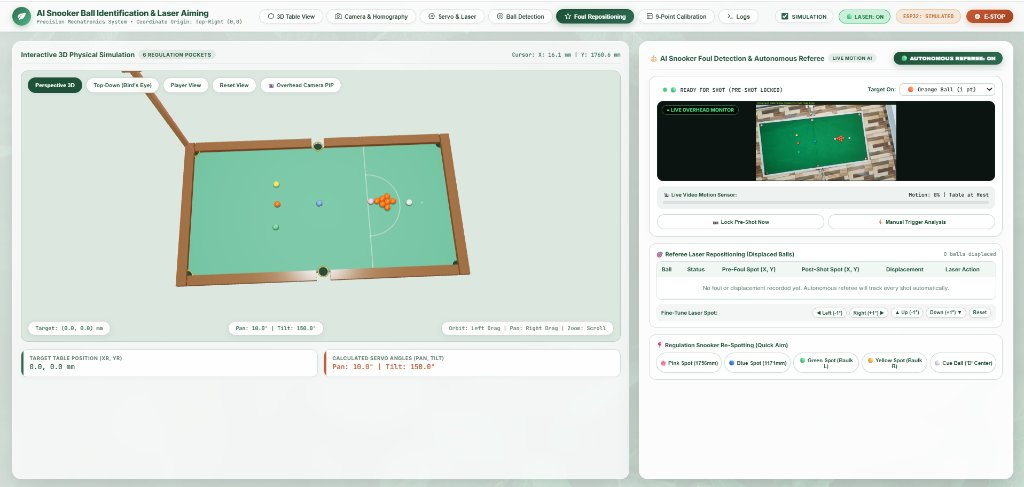
\includegraphics[width=0.46\textwidth]{ui_foul_referee.png}
\caption{Autonomous Referee UI showing motion sensor status and displaced ball table.}
\label{fig:ref_ui}
\end{figure}

\section{Hungarian Bipartite State Differencing}
Given pre-shot coordinates $\mathcal{S}_{\text{pre}} = \{ \mathbf{p}_i^{\text{pre}} \}_{i=1}^{N}$ and post-shot coordinates $\mathcal{S}_{\text{post}} = \{ \mathbf{p}_j^{\text{post}} \}_{j=1}^{M}$, we construct a cost matrix $\mathbf{C} \in \mathbb{R}^{N \times M}$ with Euclidean distances $C_{ij} = \| \mathbf{p}_i^{\text{pre}} - \mathbf{p}_j^{\text{post}} \|_2$ (and $C_{ij} = \infty$ across mismatched ball classes). Optimal assignment is solved in $O(V^3)$ time via Kuhn's Hungarian algorithm \cite{ref40}:
\begin{equation}
    \min_{\mathbf{X}} \sum_{i=1}^N \sum_{j=1}^M C_{ij} X_{ij} \quad \text{s.t.} \quad \sum_{j=1}^M X_{ij} \le 1, \; \sum_{i=1}^N X_{ij} \le 1, \; X_{ij} \in \{0, 1\}
\end{equation}
Pairs with $C_{ij} \le 10.0\,\text{mm}$ are classified as \textbf{Stationary}; pairs with $C_{ij} > 10.0\,\text{mm}$ are flagged as \textbf{Displaced} ($\mathbf{d}_i = \mathbf{p}_j^{\text{post}} - \mathbf{p}_i^{\text{pre}}$); unmatched pre-shot balls are flagged as \textbf{Potted}.

\section{Experimental Validation}
Table \ref{tab:cases} summarizes validation across four real-world match scenarios, achieving $5.2 \pm 0.8\,\text{ms}$ bipartite matching time and $100\%$ accurate state transitions.

\begin{table}[htbp]
\centering
\caption{Autonomous Ball Tracking Validation Scenarios}
\label{tab:cases}
\scriptsize
\begin{tabular}{|l|p{2.7cm}|p{2.9cm}|}
\hline
\textbf{Scenario} & \textbf{Observed Motion} & \textbf{System Classification} \\
\hline
1. Standard Miss & Cue ball moves $1840\,\text{mm}$; objects $<3.2\,\text{mm}$ & Cue: Displaced; Objects: Stationary; Foul restoration triggered \\
2. Cluster Scatter & 3 orange + 1 blue scatter ($54$--$310\,\text{mm}$) & 4 Displaced vectors isolated sequentially for restoration \\
3. Ball Pocketing & Cue ball drops into pocket (6 $\to$ 5 visible) & Cue ball flagged Potted; pre-shot spot queued \\
4. Clean Safety & Legal stroke, no foul called & Post-shot state auto-committed as next baseline \\
\hline
\end{tabular}
\end{table}

\section{Conclusion}
The proposed temporal FSM and Hungarian bipartite tracker reliably automates pre/post-shot baseline management and isolates displaced or pocketed balls without manual referee intervention, enabling rapid laser restoration.

\bibliographystyle{IEEEtran}
\begin{thebibliography}{10}
\bibitem{ref12} K. Yang, ``Single-stage snooker ball localization using deep feature pyramids,'' \textit{Sensors}, vol. 23, no. 8, p. 3945, 2023.
\bibitem{ref21} A. Deep et al., ``Multi-object tracking of cue balls with DeepSORT and Kalman filters,'' \textit{Proc. IEEE WACV}, pp. 1412--1420, 2020.
\bibitem{ref24} F. Long et al., ``Discrete-event state machine for pool robot shot selection,'' \textit{IEEE Trans. Autom. Sci. Eng.}, vol. 15, no. 4, pp. 1612--1622, 2018.
\bibitem{ref39} G. Bradski, ``The OpenCV Library,'' \textit{Dr. Dobb's Journal}, 2000.
\bibitem{ref40} H. W. Kuhn, ``The Hungarian method for the assignment problem,'' \textit{Naval Research Logistics Quarterly}, vol. 2, no. 1-2, pp. 83--97, 1955.
\end{thebibliography}

\end{document}
